\subsection{Strokes}
Strokes are a global health crisis with approximately 800,000 occurrence each year in the United States and is a leading cause of death worldwide \cite{george2017cdc} \cite{murphy2020stroke} \cite{feigin2015update}. While strokes have been decreasing worldwide, the rate of stroke in younger people (18-54 years old) has risen. The expected cause is increased hypertension, diabetes, lipid disorders, obesity, and tobacco use. 

A stroke is a medical condition where the blood vessels to the brain get blocked or burst; this means that the brain cannot get the necessary blood flow, and the tissue begins to die. There are broadly two different types of strokes \cite{perna2015rehabilitation}; ischemic strokes and hemorrhagic strokes as shown in \autoref{fig:strokes}.  An ischemic stroke is caused by obstructed blood vessels. This type of stroke accounts for approximately 85\% of all strokes. A hemorrhagic stroke is caused when the blood vessels of the brain burst.  

\begin{figure}
    \centering
    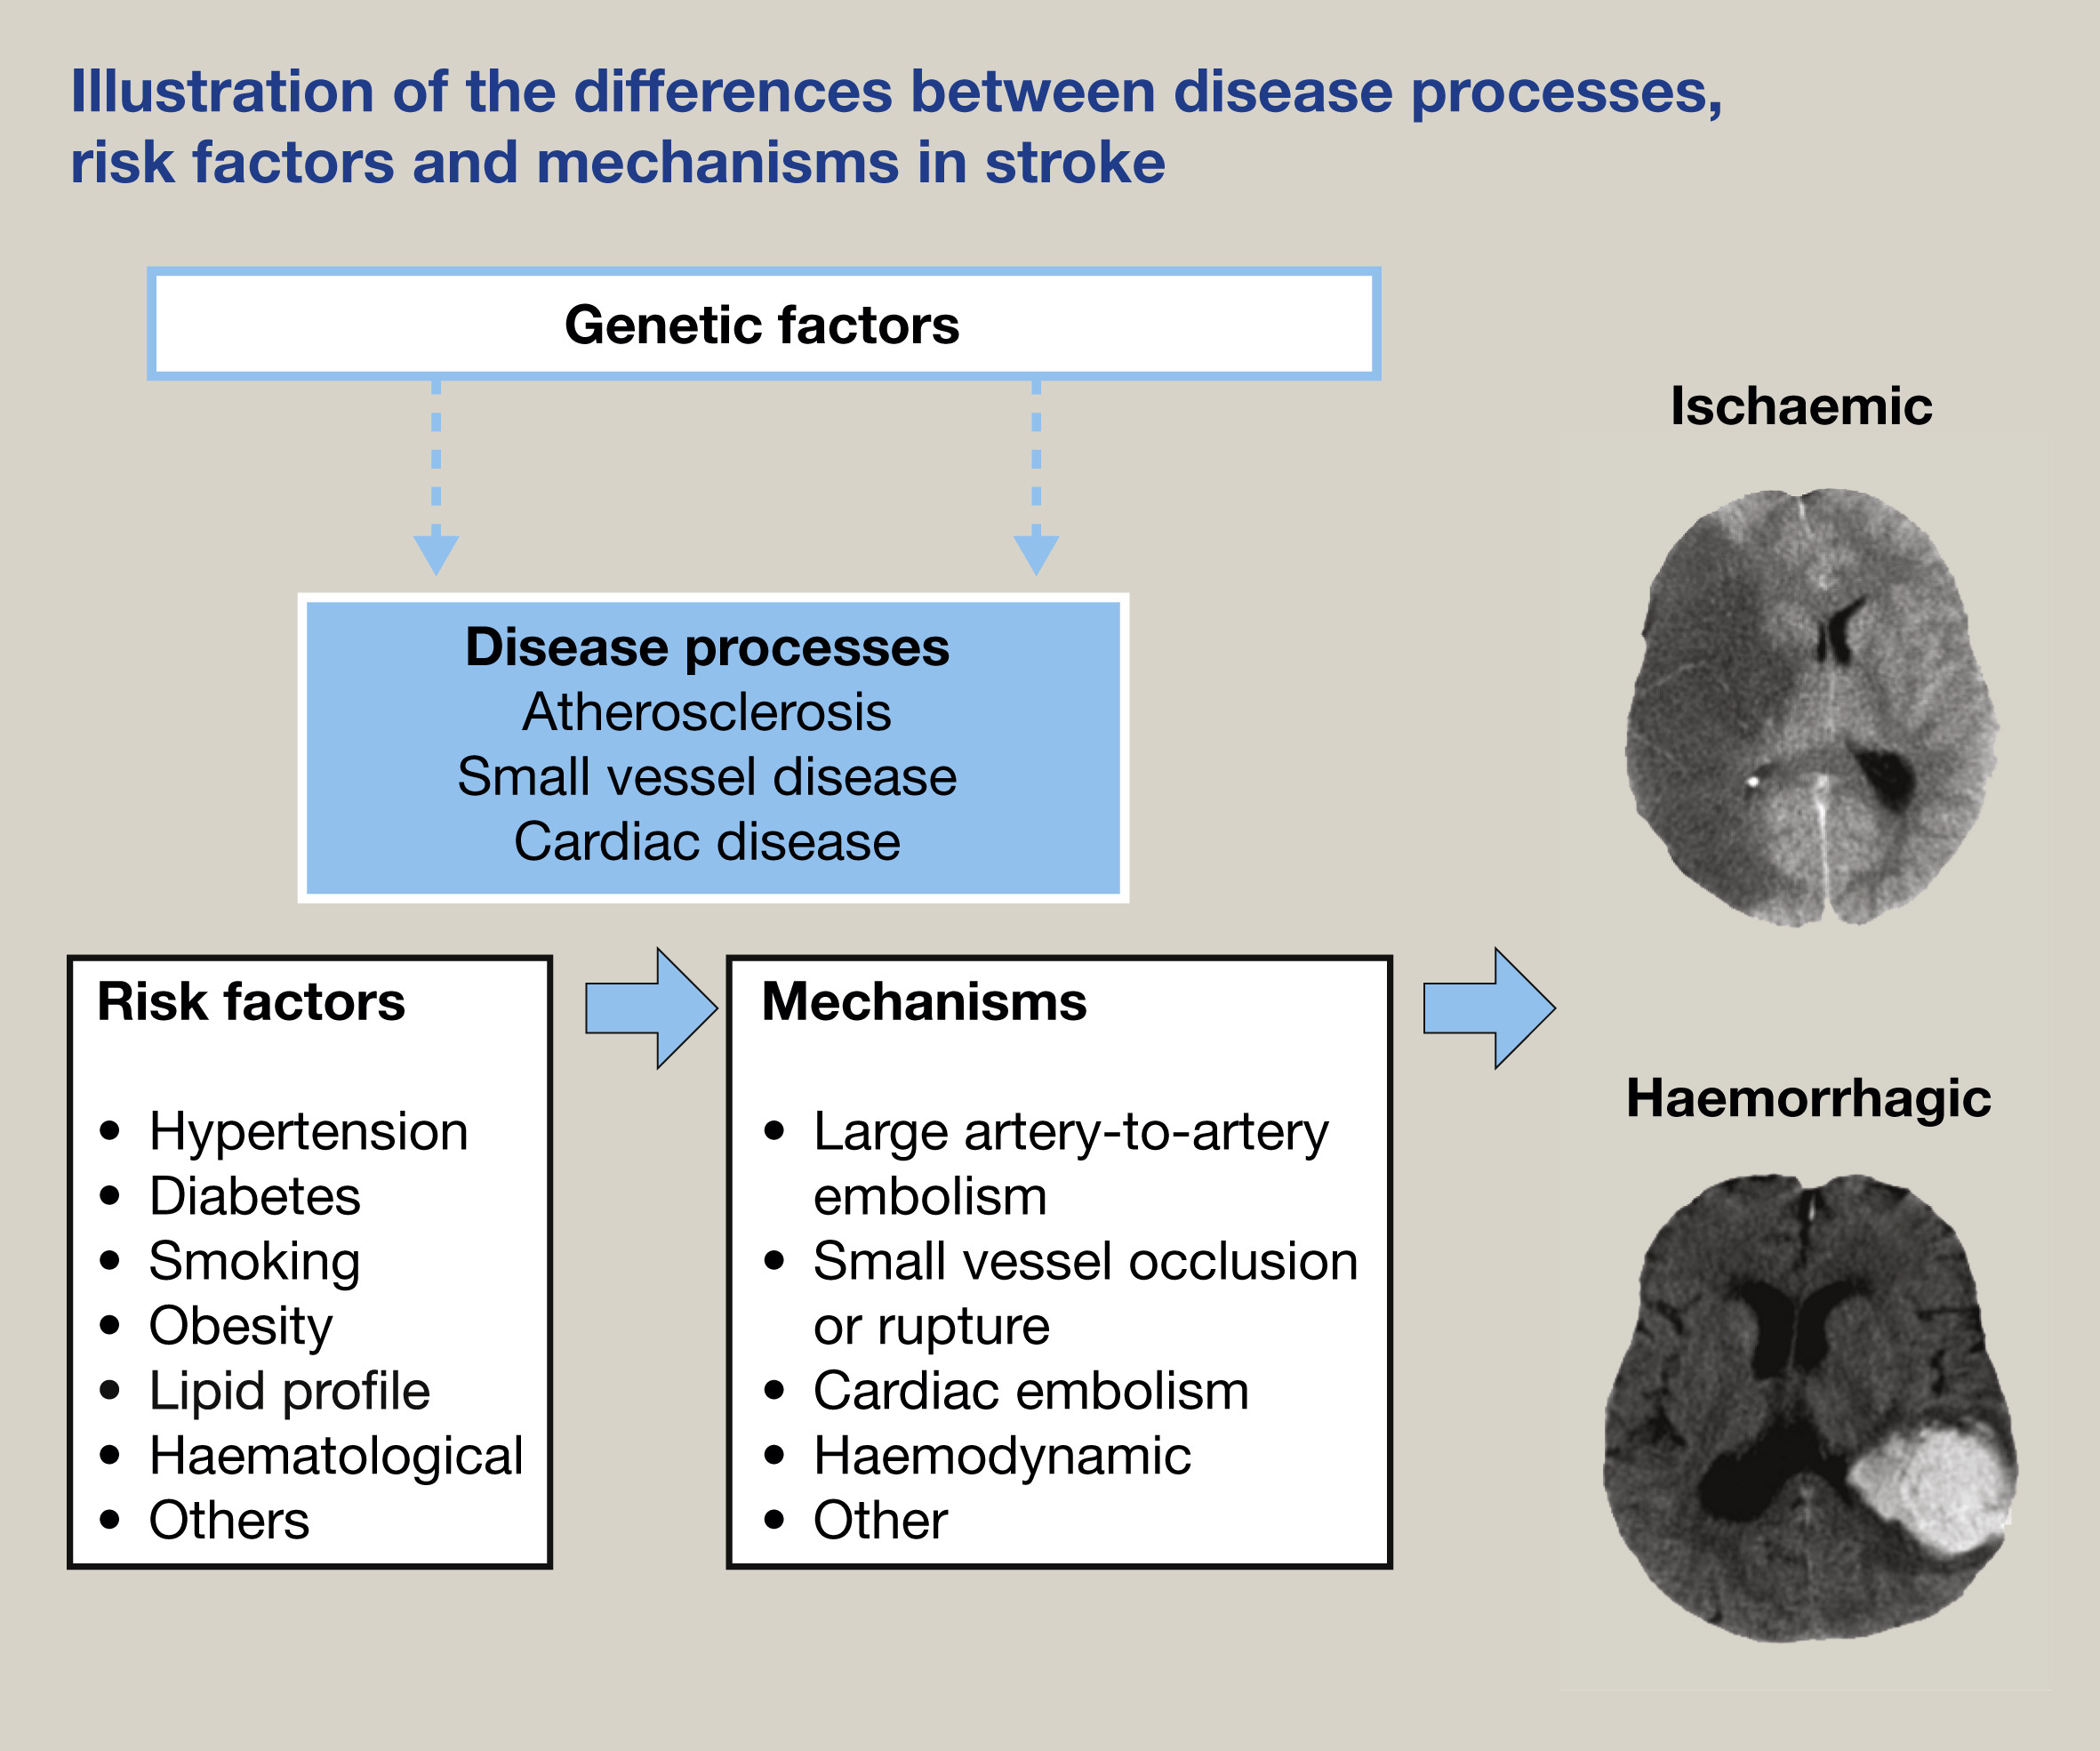
\includegraphics[scale=0.85]{images/background/stroke.jpg}
    \caption[Ischemic strokes and Hemorrhagic strokes]{Ischemic strokes and Hemorrhagic strokes \cite{murphy2020stroke}}
    \label{fig:strokes}
\end{figure}


It is crucial to receive treatment immediately after a stroke. Each minute causes more tissue and brain damage to occur \cite{saver2006time} resulting in about 1.9 million neurons per minute; this can result in both upper and lower limb weakness along with other cognitive complications \cite{pennycott2012towards}.  Emergency treatment to restore blood flow has been shown to improve outcomes which are essential for getting the patient back to normal life with less loss of functionality \cite{goyal2016endovascular}.  